%%%%%%%%%%%%%%%%%%%%%%%%%%%%%%%%%%%%%%%%%%%%%%%%%%%%%%%%%%%%%%%%%%
%%%%%%%%%%%%%%%%%%%%%%%%% PREAMBULO %%%%%%%%%%%%%%%%%%%%%%%%%%%%%%
%%%%%%%%%%%%%%%%%%%%%%%%%%%%%%%%%%%%%%%%%%%%%%%%%%%%%%%%%%%%%%%%%%
\documentclass[a4paper,10pt,twocolumn,twoside]{article}
%%% Paquetes y opciones de configuración:
%%%%%%%%%%%% Paquetes %%%%%%%%%%%%
% CODIFICACIÓN Y CONFIGURACIÓN DE PAGINA
\usepackage[utf8]{inputenc}             % Configura el Encoding (algo asi como el lenguaje interno de Latex)
\usepackage[left=2cm,right=2cm,top=2cm,bottom=2cm,headsep=0.1cm]{geometry}    % Margenes
\usepackage[spanish,es-tabla]{babel}    % Configura el Idioma a Español
\usepackage{fancyhdr}                   % Para encabezados bonitos
\usepackage{titlesec}                   % Para personalizar el titulo
% GRÁFICOS, LISTAS y TABLAS
\usepackage{graphicx}           % Para insertar figuras
\usepackage{enumerate}          % Mas control en el uso de listas
\usepackage{booktabs}           % Para tablas tipo papers
\usepackage{threeparttable}     % Mejor manejo de tablas
\usepackage[font=small,labelfont=bf,singlelinecheck=false,justification=justified]{caption}
% MATEMÁTICA
\usepackage{amsmath}            % Incorpora comodidades matematicas
\usepackage{amsfonts}           % Fuentes extras para texto matematico
\usepackage{amssymb}            % Simbolos adicionales
\usepackage{siunitx}            % Herramientas para el uso de unidades fisicas
% FORMATO Y FUENTES
\usepackage{mathptmx}           %
\usepackage{newtxtext}          %
\usepackage{newtxmath}          %
\usepackage[x11names]{xcolor}   % Permite cambiar de color el texto
\usepackage{setspace}
\usepackage{soul}               % Opciones de formato (texto tachado)
% REFERENCIAS Y GLOSARIO
\usepackage{hyperref}           % Para hipervinculos en el PDF
\usepackage{natbib}             % Controlador de biblografia (no compatible con bibtex!!!)
% OTROS
\usepackage{lipsum}             % Parrafos de texto mudo
\usepackage{fancyvrb}
\usepackage{appendix}
\usepackage{flushend}


%%%%%%%%%%%% CONFIGURACION %%%%%%%%%%%%

% Ruta de imagenes
\graphicspath{{./figures/}}

%%%%% Formato de titulos
%%% Formato Secciones
\titlespacing*{\section}{0pt}{*2}{*1}
\titleformat*{\section}{\fontsize{10pt}{10pt}\selectfont\bfseries}
%%% Formato Subsecciones
\titlespacing*{\subsection}{0pt}{*2}{*1}
\titleformat*{\subsection}{\fontsize{10pt}{10pt}\selectfont\itshape}
%%% Formato Subsubsecciones
\titlespacing*{\subsubsection}{0pt}{*2}{*1}
\titleformat*{\subsubsection}{\fontsize{10pt}{10pt}\selectfont\itshape}



%%%%% Bibliografia y Citas
%%% Carga estilo de bibliografia
\bibliographystyle{bibstyle}
%%% Cambia el titulo de la seccion de bibliografia
\addto\captionsspanish{\def\bibname{Referencias}}
%%% Cambia el estilo de las citas
\setcitestyle{authoryear,open={(},close={)}}
\bibpunct{\textcolor{blue}{(}}{\textcolor{blue}{)}}{,}{a}{}{;}

%%%%%  Hipervinculos
%%% Estilo de hipervinculos
\hypersetup{
    colorlinks = true,
    linkcolor = {black},
    citecolor = {blue},
    urlcolor = {blue},
    anchorcolor = {green},
    filecolor = {orange},
    menucolor = {red},
    runcolor = {cyan}
}

% Cambio de margenes
\newenvironment{changemargin}[2]{%
\begin{list}{}{%
\setlength{\topsep}{0pt}%
\setlength{\leftmargin}{#1}%
\setlength{\rightmargin}{#2}%
\setlength{\listparindent}{\parindent}%
\setlength{\itemindent}{\parindent}%
\setlength{\parsep}{\parskip}%
}%
\item[]}{\end{list}}

%%%%%%%%%%%%%%%%%%% ENCABEZADO Y PIE DE PAGINA %%%%%%%%%%%%%%%%%%%
\pagestyle{fancy} % El estilo de pagina es el indicado por el paquete fancyhdr
\fancyhf{} % Limpia el encabezado y pie de pagina
\fancyhead[LE,RO]{\thepage}
\fancyhead[RE]{\fontsize{10pt}{0}\selectfont \textsc{Abril 2021}}
\fancyhead[CE]{\fontsize{12pt}{0}\selectfont \so{\textsc{Nahuel G\'omez}}}
\fancyhead[LO]{\fontsize{10pt}{0}\selectfont \textsc{Informe N\textdegree 1}}
\fancyhead[CO]{\fontsize{12pt}{0}\selectfont \so{\textsc{Asignatura}}}
\renewcommand{\headrulewidth}{0pt} % Remueve la línea del encabezado

%%%%%%%%%%%%%%%%%%%%%%%%%%%% título %%%%%%%%%%%%%%%%%%%%%%%%%%%%%%
% título
\title{
    \fontsize{14pt}{16pt}\selectfont
    \textbf{
        Plantilla para Informes 
        Académicos en \LaTeX
    }
}
% Autores
\author{
\fontsize{10pt}{8pt}\selectfont
    \textsc{
        Nahuel Gómez$^1$
    }
}
% Afilaciones, contacto y fecha de publicacion
\date{
\fontsize{9pt}{9pt}\selectfont
\textit{
$^1$Centro de Investigación del Mar y la Atmósfera, Universidad de Buenos Aires, Buenos Aires, Argentina\\[2ex]
}
Correspondencia: \href{mailto:mail@gmail.com}{\texttt{mail@gmail.com}} \\ [1ex]
Publicado \today
}


%%%%%%%%%%%%%%%%%%%%%%%%%%%%%%%%%%%%%%%%%%%%%%%%%%%%%%%%%%%%%%%%%%
%%%%%%%%%%%%%%%%%%%%%%%%%% CUERPO %%%%%%%%%%%%%%%%%%%%%%%%%%%%%%%%
%%%%%%%%%%%%%%%%%%%%%%%%%%%%%%%%%%%%%%%%%%%%%%%%%%%%%%%%%%%%%%%%%%

\begin{document}

%%%%%%%%%%%%%%%%%%%%%%%%%%% RESUMEN %%%%%%%%%%%%%%%%%%%%%%%%%%%%%%
\twocolumn[
  \begin{@twocolumnfalse}
    \maketitle
    \thispagestyle{fancy}
    \begin{abstract}
        Esta plantilla de \LaTeX{} está orientada a escribir informes universitarios y tiene cargada las librerías necesarias para escribir con practicidad y prolijidad elementos recurrentes como ecuaciones, figuras, tablas, referencias bibliográficas, etc. Se utiliza la clase \texttt{article} con la opción \texttt{twoside} para que el texto se vea en doble columna. Se utiliza natbib para administrar la base de datos bibliográfica.
       \vspace*{0.5cm}
    \end{abstract}
  \end{@twocolumnfalse}
]

%%%%%%%%%%%%%%%%%%%%%%%%%%% CONTENIDO %%%%%%%%%%%%%%%%%%%%%%%%%%%%
\section{Contenido}

Esta plantilla consta de los siguientes archivos:
\begin{itemize}
    \item \texttt{main.tex} es el documento principal y se divide en dos partes. Por un lado, el preámbulo es donde se cargan los paquetes, se realizan las configuraciones y se escriben el título, autores, etc. En esta plantilla los paquetes y las configuraciones están en un archivo aparte y se lo llama con el comando \verb+\input{}+. Por otro lado, en el cuerpo se escribe todo el contenido del artículo: el resumen (abstract) y las secciones. Las referencias bibliográficas se tratan a parte.
    \item \texttt{packages.tex} es el archivo aparte donde están cargados todos los paquetes (o librerías) utilizados. También se hacen configuraciones referidas a los margenes, bibliografía, estilo de citas, estilos de hipervínculos, formato de encabezados de sección, etc. Si querés agregar un paquete o personalizar algunos aspectos de la plantilla deberías hacerlo acá. En caso contrario, no es necesario que modifiques este archivo.
    \item \texttt{bibstyle.bst} es el estilo de la bibliografía. Es una traducción al español del estilo empleado por las revistas y el boletín de la \emph{American Meteorological Society}. Este estilo emplea el paquete \texttt{natbib}, por lo que utiliza \texttt{BibTeX} para procesar la base de datos bibliográfica.
    \item \texttt{references.bib} es la base de datos bibliográfica, con algunos ejemplos de como debe editarse.
    \item \texttt{template.tex} una versión en limpio de \texttt{main.tex} lista para ser editada.
    \item En la carpeta \texttt{figures} se guardan las figuras que se utilizan en el documento.
\end{itemize}

\section{Cuestiones generales}
Se utiliza la clase \texttt{article}, la más común de \LaTeX. Mi intención es generar una plantilla para informes en formato de dos columnas que sea prolija y \emph{práctica}. Esto último es fundamental. Hay muchas opciones para generar un artículo de dos columnas, quizás la más conocida es usando el paquete \texttt{multicols}. Sin embargo, fue una gran desilusión cuando me di cuenta de que este paquete no admite elementos flotantes (figuras, tablas, etc) que abarquen las dos columnas. Para mi esto es fatal porque a veces requiero insertar paneles con muchos campos y necesito disponer de todo el ancho de la hoja. Esto es posible usando la opción \texttt{twocolumn} cuando definimos la clase del documento:
\begin{Verbatim}[fontsize=\fontsize{7pt}{7pt}\selectfont]
\documentclass[a4paper,10pt,twocolumn,twoside]{article}
\end{Verbatim}
Si bien ganamos practicidad, perdemos algo de la prolijidad que nos brinda el paquete \texttt{multicols}.

También se define un tamaño de letra de 10 puntos y un tamaño de hoja A4. Por otro lado, el paquete \texttt{mathptmx} define a Adobe Times Roman como tipo de letra por defecto; además \texttt{newtxtext} y \texttt{newtxmath} ofrecen algunas opciones de formato adicionales. Los márgenes se configuran con el paquete \texttt{geometry} y son de \SI{2}{\cm} en todos los lados. El idioma español se define con el paquete \texttt{babel} y se especifica que se use <<Tabla>> y no <<Cuadro>> en la leyenda de estos elementos. (Por cierto, cuando se configura el idioma español, es mejor el empleo de las <<comillas españolas>> por sobre las ``comillas inglesas''). Algunos paquetes se cargan para ofrecer opciones de formato adicionales: \texttt{xcolor} permite cambia el {\color{red}color} del texto (ver \href{https://ctan.dcc.uchile.cl/macros/latex/contrib/xcolor/xcolor.pdf}{documentación}) mientras que \texttt{soul} permite \ul{subrayar} y \st{tachar} el texto (comandos \verb+\ul{}+ y \verb+\st{}+ respectivamente).  

Por último, el paquete \texttt{titlesec} habilita los comandos \verb+\titlespacing+ y \verb+\titleformat+ para controlar el tamaño de fuente y el espaciamiento de los títulos de secciones, subsecciones, etc. Esto se encuentra en la parte de configuración del archivo \texttt{packages.tex} de la siguiente forma:
\begin{Verbatim}[fontsize=\fontsize{8pt}{8pt}\selectfont]
%%%%% Formato de titulos
%%% Formato Secciones
\titlespacing*{\section}{0pt}{*2}{*1}
\titleformat*{\section}
{\fontsize{10pt}{10pt}\selectfont\bfseries}
%%% Formato Subsecciones
\titlespacing*{\subsection}{0pt}{*2}{*1}
\titleformat*{\subsection}
{\fontsize{10pt}{10pt}\selectfont\itshape}
%%% Formato Subsubsecciones
\titlespacing*{\subsubsection}{0pt}{*2}{*1}
\titleformat*{\subsubsection}
{\fontsize{10pt}{10pt}\selectfont\itshape}
\end{Verbatim}
Tanto \verb+\titlespacing+ como \verb+\titleformat+ tienen un asterisco (*), esto indica que se está utilizando la versión <<abreviada>> del comando (ver \href{https://ctan.dcc.uchile.cl/macros/latex/contrib/titlesec/titlesec.pdf}{documentación}). El primer argumento de ambos comandos indica que título se quiere formatear (secciones, subsecciones, etc). En \verb+\titlespacing+ el segundo argumento es la identación izquierda del título, mientras que el tercer y el cuarto argumento indican el interlineado anterior y posterior del título, respectivamente. Es importante que mantengas el asterisco delante de estos números, esto fuerza un determinado tipo de unidad, pero una sintaxis simplificada, torturate con la documentación si querés más detalles. Por otro lado, en \verb+\titleformat+ en el segundo argumento indicamos como queremos formatear al título. Con \verb+\fontsize{}{}+ le indicamos el tamaño de la fuente (primer argumento) y el interlineado entre las líneas del título (segundo argumento). Luego es obligatorio colocar \verb+\selectfont+ para aplicar el formato. La ultima opción indica que tipo de letra queremos usar \verb+\bfseries+ para \textbf{negritas} y \verb+\itshape+ para \textit{itálicas} (ver \href{https://www.overleaf.com/learn/latex/Font_sizes,_families,_and_styles}{otras opciones}).

\section{Texto preliminar}

\subsection{Título, autores y afiliaciones}
El título y los autores se modifican en la parte final del preámbulo en el archivo \texttt{main.txt}. La referencia entre autores y afiliaciones se hace de manera manual utilizando \verb+$^1$+. En lo personal considero muy exagerado recurrir a un paquete adicional para hacer colocar las afiliaciones (como he visto en varias ocasiones). Hay una opción sucia, pero rápida y efectiva, que es colocar las afiliaciones dentro del comando \verb+\date{}+:
\begin{Verbatim}[fontsize=\fontsize{7pt}{7pt}\selectfont]
% Afilaciones, contacto y fecha de publicacion
\date{
\fontsize{9pt}{9pt}\selectfont
\textit{
$^1$Centro de Investigación del Mar y la Atmósfera,
Universidad de Buenos Aires, Buenos Aires, Argentina\\[2ex]
}
Correspondencia: 
\href{mailto:mail@gmail.com}{\texttt{mail@gmail.com}} \\ [1ex]
Publicado \today
}
\end{Verbatim}
Como se ve, abusamos y también ponemos de yapa un email de contacto. Es importante que no te olvides de colocar el marcador \verb+\\+ para hacer un salto de línea y el interlineado \verb+[#ex]+, puesto que \LaTeX{} no realiza esto de manera automática dentro de este comando. En el archivo \texttt{template.tex} se muestra cómo se modifica la escritura cuando hay más autores.

\subsection{Encabezados: numero de página y otras yerbas}
El paquete \texttt{fancyhdr} permite manipular los encabezados y los pies de página. Yo prefiero que solo haya encabezado, puesto que los pie de página a veces se chocan con las notas al pie. Cuando definí la clase a usar configure la opción \texttt{twoside}. Esto es para que los encabezados se alternen entre páginas pares e impares. También incluí la configuración del encabezado en el archivo \texttt{main.tex} porque seguramente vas a querer adaptarlo a tus necesidades. No voy a explicar como modificarlo porque en \emph{Overleaf} hay una guía sencilla y corta de como hacerlo: \href{https://es.overleaf.com/learn/latex/headers_and_footers}{headers and footers}. Si voy a explicar algunas particularidades de la plantilla. Por defecto, el encabezado tiene una línea horizontal que lo separa del resto de la página, agregué una línea para que esto no ocurra (si querés que aparezca solamente tenpes que borrarla). Para que el texto central se vea en \href{https://es.wikipedia.org/wiki/Versalita}{\textsc{versalita}} usamos el comando \verb+\textsc{}+ y para que las letras se vean más espaciadas usamos el comando \verb+\so{}+ del paquete \texttt{soul}. Es importante aclarar que los comandos de este paquete no entienden las letras con tilde, hay que indicárselos manualmente: \verb+G\'omez+.

\subsection{El resumen}
Acá es donde hacemos nuestro primer sacrificio al no usar el paquete \texttt{multicol}. Por defecto, esta librería se encarga de que el resumen aparezca centrado, con un margen más amplio y por encima del contenido principal. Cuando usamos la clase \texttt{article} con la opción \texttt{twocolumn}, el resumen se coloca por defecto dentro del cuerpo del texto, como si fuese una sección más. Para hacer que aparezca como en el paquete \texttt{multicol} usamos el siguiente codigo:
\begin{Verbatim}[fontsize=\fontsize{7pt}{7pt}\selectfont]
\twocolumn[
  \begin{@twocolumnfalse}
    \maketitle
    \thispagestyle{fancy}
    \begin{abstract}
       Texto ...
       \vspace*{0.5cm}
    \end{abstract}
  \end{@twocolumnfalse}
]
\end{Verbatim}
Si me preguntan como funciona esto, no tengo idea, si me preguntan de donde lo saque, no lo recuerdo. \LaTeX{} es a veces muy misterioso. Créditos a la criatura que se le ocurrió. Dentro de este entorno colocamos el comando \verb+\thispagestyle{fancy}+ para indicar que la primera página tiene encabezado (por defecto no lo lleva nunca). Al final colocamos un interlineado por debajo del resumen usando: \verb+\vspace*{0.5cm}+. Entonces, asi logramos reproducir el texto inicial de un artículo en dos columnas sin recurrir a paquetes extras que nos puedan traer problemas con elementos flotantes que son de suma importancia.

\section{Elementos Flotantes}

En el paquete \texttt{multicols} uno obtiene el texto en dos columnas escribiéndolo dentro del entorno:
\begin{Verbatim}[fontsize=\fontsize{7pt}{7pt}\selectfont]
\begin{multicols}{2}
Texto ...
\end{multicols}
\end{Verbatim}
Sin embargo, cuando uno quiere insertar un elemento flotante (tabla o figura) que ocupe el ancho de las dos columnas se tiene que interrumpir este entorno, insertar el elemento flotante y volverlo a abrir. Esto tiene como consecuencia que la figura no <<flote>> en el texto, y quede ubicada donde uno exactamente indicó. Si, por ejemplo, queremos que la imagen aparezca en la parte superior de la página, debemos hacer mediciones milimétricas para determinar donde cortar el texto e insertar la figura (y el resultado de esto no siempre es prolijo). O sea, debemos colocar la figura manualmente. Y el punto es: ¿por que no usar directamente Microsoft Word si nos gusta acomodar figuras manualmente? Por esto usamos la opcion \texttt{twocolumn} de la clase \texttt{article}. Esto nos permite utilizar los entornos \texttt{figure} y \texttt{table} para elementos flotantes que ocupen el ancho de \emph{una sola columna} y los entornos \texttt{figure*} y \texttt{table*} para los elementos que abarquen \emph{ambas columnas}.

\subsection{Tablas}

\begin{table}[b]
    \centering
    \caption{Valores aceptados para la velocidad de la luz y la constante de Boltzmann.}
    \label{tab:tabla_1}
    \resizebox{0.5\textwidth}{!}{
    \begin{tabular}{cc}
        \toprule[1pt]
        Magnitud & Valor\\
        \midrule
        \ \ Velocidad de la luz (\si{m\per s}) & \num{2.997925e8}\\
        \ \ Constante de Boltzmann (\si{\joule\per\K}) & \num{1.380658e-23}\\
        \bottomrule[1pt]
    \end{tabular}
    }
\end{table}

\begin{table*}[t]
    \centering
    \resizebox{0.8\textwidth}{!}{
        \begin{threeparttable}
            \caption{Lista de reanálisis}
            \label{tab:tabla_2}
            \begin{tabular}{ccccc}
                \toprule[1pt]
                Nombre & Periodo & Referencia & Nivel más alto (\si{\hecto\Pa}) & Resolucion reticular (\textdegree)\tnote{1} \\
                \midrule
                ERA-Interim & 1979-2016 & Dee et al. (2011) & 1 & 2,5 \\
                NCEP-NCAR & 1958-2016 & Kalnay et al. (1996) & 10 & 2,5 \\
                CSFR\tnote{a}  & 1979-2016 & Saha et al. (2010, 2014) & 1 & 2,5 \\
                JRA-55 & 1958-2016 & Kobayashi et al. (2015) & 1 & 1,25 \\
                MERRA-2 & 1980-2016 & Gelaro et al. (2017) & 0,1 & 1,25 \\
                \bottomrule[1pt]
            \end{tabular}
            \begin{tablenotes}
                \item [1] Una nota al pie de la tabla...
                \item [a] Otra nota más.
            \end{tablenotes}
        \end{threeparttable}
    }
\end{table*}

En la Tabla \ref{tab:tabla_1} es un ejemplo de una tabla que abarca solo una columna. Si te preguntas como se logra que se acomode tan finamente al ancho es porque estamos usando el entorno \texttt{tabular} dentro del comando \texttt{risezebox}:
\begin{Verbatim}[fontsize=\fontsize{7pt}{7pt}\selectfont]
\resizebox{0.5\textwidth}{!}{
    \begin{tabular}
        Tabla ...
    \end{tabular}
}
\end{Verbatim}
Nota que le indicamos específicamente que ocupe el 50\% del ancho del texto (que es el ancho de las \emph{dos} columnas, el espacio intermedio no cuenta). Podrías ponerle que ocupe un espacio menor, la tabla ajustará sus dimensiones para caber en el espacio que le indiques. Por otro lado, la Tabla \ref{tab:tabla_2} emplea el entorno \texttt{table*}, por lo que abarca <<todo>> el ancho del texto (en realidad le puse un 80\% usando el comando \verb+\resizebox+). Hay algunas cuestiones estéticas que vale la pena remarcar. Estoy usando las líneas horizontales del paquete \texttt{booktabs} (comandos \verb+\toprule+, \verb+\midrule+ y \verb+\bottomrule+). Por otro lado, estoy haciendo uso intensivo del paquete \texttt{caption}. Con este paquete hacemos que la letra de la leyenda sea más pequeña de lo normal (opción \texttt{font=small}), que la etiqueta aparezca en negritas (\texttt{labelfont=bf}) y que el texto esté justificado (\texttt{justification=justified}). Además, por defecto \LaTeX{} hace que las leyendas que abarquen una única línea aparezcan centradas, para evitar esto ponemos la opción: \texttt{singlelinecheck=false}. Le estamos dando dos usos al paquete \texttt{threeparttable}. Primero, hacemos que la leyenda aparezca alineada a la tabla y no al texto (como en la Tabla \ref{tab:tabla_2}). Esto lo hacemos colocando el comando \verb+\caption{}+ dentro del entorno \texttt{threeparttable}. Segundo, lo usamos para colocar notas al pie de tabla, haciendo de este un problema totalmente trivial. Usamos \verb+\tnote{#}+ para indicar las notas y en el entorno \texttt{tablenotes}, después del entorno \texttt{tabular}, para escribir nuestras notas (la \href{https://ctan.dcc.uchile.cl/macros/latex/contrib/threeparttable/threeparttable.pdf}{documentación} es corta, por lo que te recomiendo leerla). Un esquema:
\begin{Verbatim}[fontsize=\fontsize{7pt}{7pt}\selectfont]
\begin{table*}
    \centering
    \resizebox{0.8\textwidth}{!}{
        \begin{threeparttable}
            \caption{Una leyenda}
            \label{referencia}
            \begin{tabular}
                Una tabla... con \tnote{a}
            \end{tabular}
            \begin{tablenotes}
                \item[a] Notas al pie de la tabla
            \end{tablenotes}
        \end{threeparttable}
    }
\end{table*}
\end{Verbatim}

\subsection{Figuras}
Las figuras son los elementos flotantes más importantes. La idea es la misma que para las tablas, usamos el entorno \texttt{figure} para figuras que abarquen solo una columna (ej. Figura \ref{fig:figura_1}) y usamos el entorno \texttt{figure*} para figuras que abarquen ambas columnas (ej. Figura \ref{fig:figura_2}). También podemos estar interesados en incluir una figura de gran tamaño, por lo que podemos incluir la opción \texttt{[p]} en el entorno \texttt{figure*} (es una elemento que abarca ambas columnas por lo que tenés que usar el entorno con asterisco). La Figura \ref{fig:figura_3} es un ejemplo de esto. También es posible hacer lo mismo con el entorno \texttt{table*}. No está de más decir que el paquete \texttt{graphicx} nos da todas las facilidades para incluir figuras.

Tanto en las tablas como en las figuras hemos usado el paquete \texttt{siunitx} para escribir los valores numéricos en notación científica y con unidades físicas. Recomiendo fuertemente leer la \href{https://ctan.dcc.uchile.cl/macros/latex/contrib/siunitx/siunitx.pdf}{documentación} para ver todas las posibilidades.

\begin{figure}[b]
    \centering
    \includegraphics[width=0.5\textwidth]{HSvsHN.png}
    \caption{Climatologías mensuales (1979-2018, sin 2002) en \SI{10}{\hecto\Pa} de la vorticidad potencial (sombreado, 1 PVU $= 10^{-6}$ \si{K.m^2.kg^{-1}.s^{-1}}) y la altura geopotencial (contornos, en \si{\km}); para (izquierda) agosto en el HS y (derecha) enero del HN.}
    \label{fig:figura_1}
\end{figure}

\begin{figure*}[t]
    \centering
    \includegraphics[width=0.8\textwidth]{ozone_hole.png}
    \caption{Promedios diarios de la columna total de ozono en unidades Dobson para los días indicados. La isolínea de 220 UD se muestra en celeste punteado.}
    \label{fig:figura_2}
\end{figure*}

\begin{figure*}[p]
    \centering
    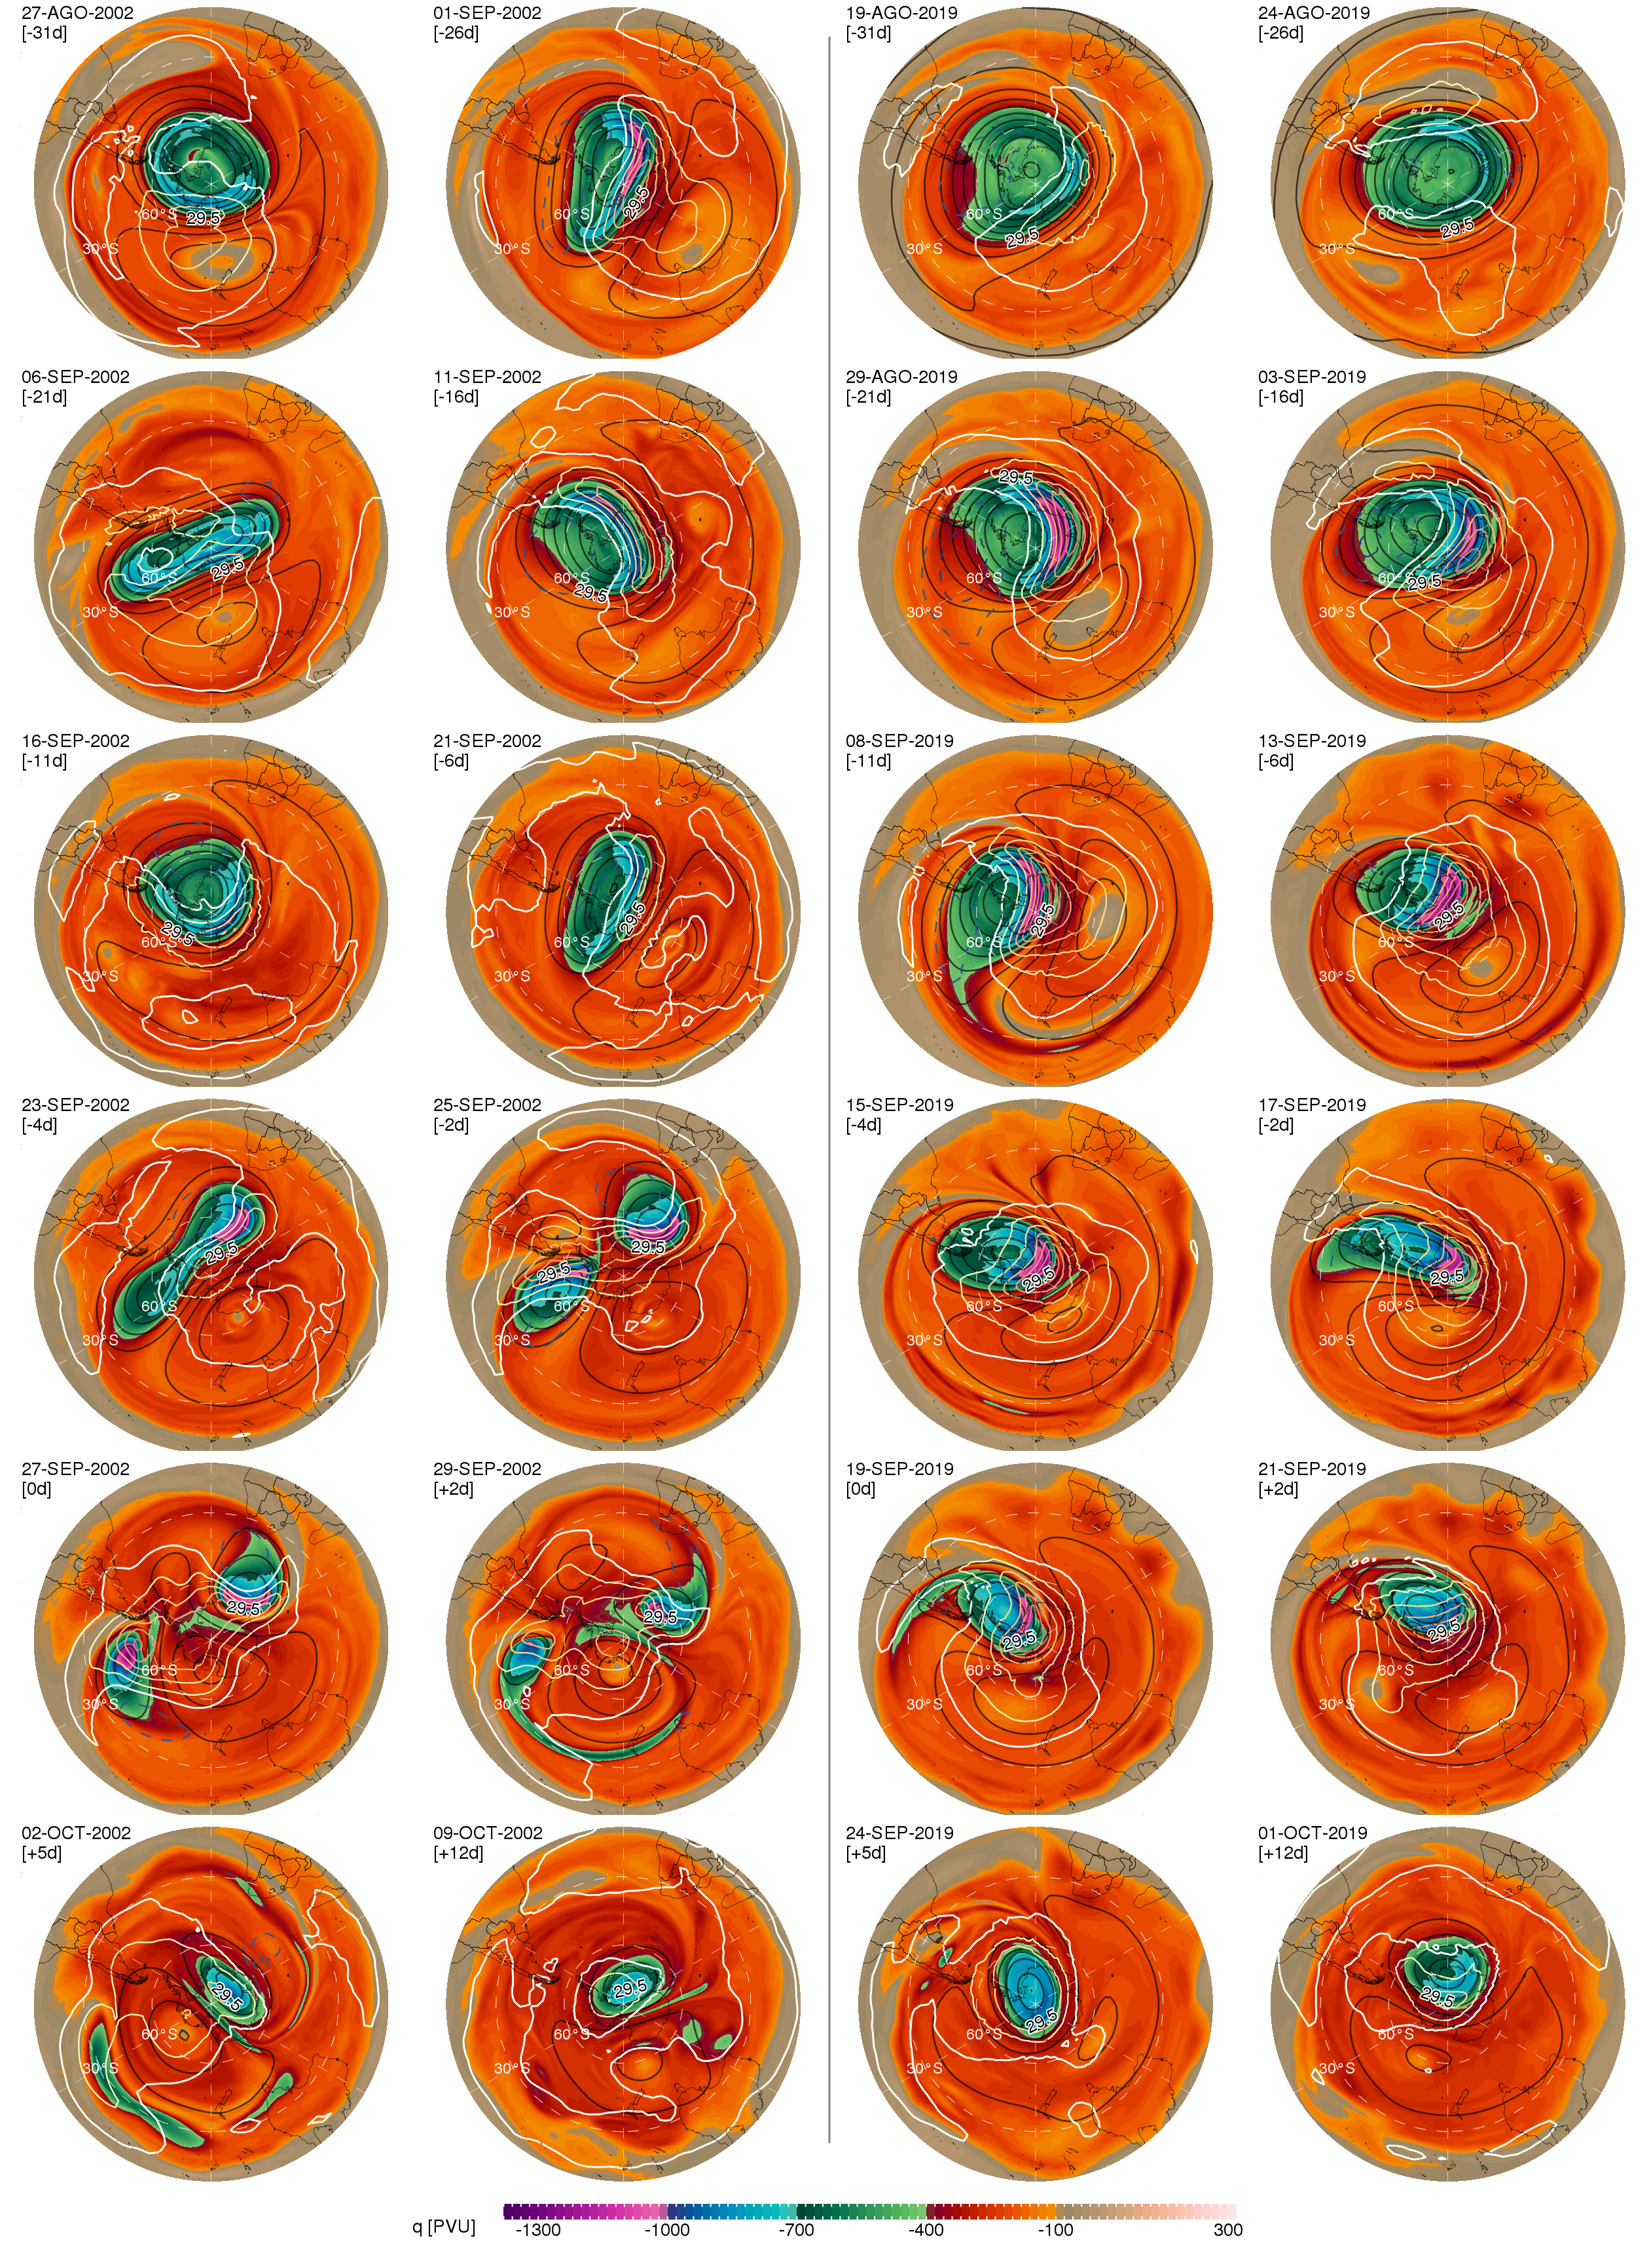
\includegraphics{horiz_field_10hpa.png}
    \caption{Series de campos horizontales en \SI{10}{\hecto\Pa} de $q$ (sombreado), $Z$ (contornos negros, cada \SI{500}{\meter}) y anomalía de $T$ (contornos coloreados, cada \SI{10}{\degreeCelsius}), en días seleccionados de agosto, septiembre y octubre del 2002 (1ra y 2da columna) y del 2019 (3ra y 4ta columna). Se muestra el valor de la isohipsa de \SI{29,5}{\km}. La isoterma de \SI{0}{\degreeCelsius} se muestra como una línea blanca gruesa.}
    \label{fig:figura_3}
\end{figure*}

\section{Ecuaciones}
Las ecuaciones largas y los artículos en dos columnas son enemigos naturales (como los escoceses y los japoneses). Para esto hay dos opciones clasicas. Primero usar el comando \verb+\resizebox{}{}{$$}+ (y no nos debemos olvidar de colocar la ecuacion entre signos \$, \emph{aun} dentro del entorno \texttt{equation}):

\begin{equation}
    \resizebox{0.44\textwidth}{!}{$\frac{\partial\mathbf{V}}{\partial t} = -\mathbf{V}\cdot\nabla\mathbf{V}-\frac{1}{\rho}\nabla P+\mathbf{g}-2\Omega\times\mathbf{V}-\Omega\times\left(\Omega\times\mathbf{r}\right)+\nu\nabla^2\mathbf{V}+\frac{1}{3}\nu\nabla\left(\nabla\cdot\mathbf{V}\right)$}
\end{equation}

La segunda opción es usar el entorno \texttt{aling} para partir la ecuación. Esto no siempre es posible porque por ahi las expresiones en si son muy largas (como integrales o sumatorios), en ese caso es quizás es más útil el comando \verb+\resizebox+. En ese caso obtenemos:
\begin{align}
\begin{split}
    \frac{\partial\mathbf{V}}{\partial t} & = -\mathbf{V}\cdot\nabla\mathbf{V}-\frac{1}{\rho}\nabla P+\mathbf{g} \\
     & - 2\Omega\times\mathbf{V}-\Omega\times\left(\Omega\times\mathbf{r}\right) \\
     & + \nu\nabla^2\mathbf{V}+\frac{1}{3}\nu\nabla\left(\nabla\cdot\mathbf{V}\right)
\end{split}
\end{align}
Notar que dentro del entorno \texttt{aling} usamos el entorno \texttt{split} para que numere una única vez a la ecuación (y no cada línea por separado). El entorno \texttt{split} nos garantiza el alineamiento vertical de la numeración. Estos entornos, y los símbolos matemáticos, son provistos por los paquetes \texttt{amsmath}, \texttt{amsfonts} y \texttt{amssymb}.

\section{Hipervínculos}

Los hipervínculos se habilitan usando el paquete \texttt{hyperref}. Entendemos por esto a los vínculos internos (las referencias de ecuaciones, figuras, tablas y bibliografía) y los externos (páginas web). Es posible modificar el color de los hipervínculos usando el comando \verb+\hypersetup+, yo deje las referencias externas y la bibliografía en azul y el resto en negro (hay otras posibilidades pero jamas les he dado uso).

\subsection{Páginas web}
Hay dos comandos para insertar páginas web: \verb+\url{}+, que muestra la dirección completa, y \verb+\href{}{}+, en el primer argumento ponemos la dirección y en el segundo un texto que se mostrará en su lugar. Ya di varios ejemplos de esto a lo largo del texto.

\subsection{Bibliografía}

Como dije en la primera sección, esta plantilla usa el estilo de bibliografía que usan las revistas y el boletín de la \emph{American Meteorological Society}. Este estilo esta configurado en el archivo \texttt{bibstyle.bst} y asume que se está utilizando el paquete \emph{natbib}. La documentación de Overleaf cuenta con una sección sobre \href{https://www.overleaf.com/learn/latex/bibliography_management_with_natbib}{cómo administrar la bibliografía con natbib}. Es importante aclarar que \texttt{natbib} no es compatible con \texttt{biber}, requiere el uso de \texttt{BibTex} para procesar la base de datos bibliográfica. Si no entendés la diferencia entre \texttt{natbib}, \texttt{BibLaTeX}, \texttt{biber} y \texttt{BibTeX} te recomiendo que leas el siguiente artículo en \emph{Stack Exchange}: \href{https://tex.stackexchange.com/questions/25701/bibtex-vs-biber-and-biblatex-vs-natbib}{bibtex vs. biber and biblatex vs. natbib}. En caso de que quieras usar otro estilo simplemente tenés que reemplazar el archivo \texttt{bibstyle.bst} por el que quieras usar. Para cargar el estilo usamos el comando \verb+\bibliographystyle{bibstyle}+ dentro del archivo \texttt{packages}.

En el archivo \texttt{references.bib} dejo ejemplos de como cargar referencias a libros \citep{ANDREWS1987,HOLTON2004}, artículos en revistas \citep{BALDWINetal2020-11}, artículos en libros \citep{PLUMB2010}, artículos en un libro multivolumen \citep{ONEILLetal2015}, tesis \citep{CLARK2017-11}, reportes técnicos \citep{LIMetal2020-1}. Algunas cuestiones referidas al estilo se pueden controlar con los comandos:
\begin{Verbatim}[fontsize=\fontsize{7pt}{7pt}\selectfont]
\addto\captionsspanish{\def\bibname{Referencias}}
\setcitestyle{authoryear,open={(},close={)}}
\bibpunct{\textcolor{blue}{(}}{\textcolor{blue}{)}}{,}{a}{}{;}
\end{Verbatim}
La primera línea cambia el titulo de la sección <<Bibliografía>> por <<Referencias>>. La segunda línea es para establecer el orden autor-año y que use paréntesis como elemento separador (podríamos usar corchetes si queremos). La tercera línea es para que los elementos separadores aparezcan del mismo color que el que pusimos en \verb+\hypersetup{}+. Por supuesto, para que las referencias aparezcan debidamente debemos incluir el comando:
\begin{Verbatim} [fontsize=\fontsize{7pt}{7pt}\selectfont]
\bibliography{references}
\end{Verbatim}
al final del archivo \texttt{main.tex}.

%%%%%%%%%%%%%%%%%%%%%%%%%%%% APENDICE %%%%%%%%%%%%%%%%%%%%%%%%%%%% 
\appendix
\vspace{1ex}
\begin{center}
    \so{\textsc{AP\'ENDICE}}
\end{center} 

\section{Paquetes adicionales}
El apéndice se agrega usando el comando \verb+\appendix+, luego de esto todas las secciones aparecen señaladas con letras. Por defecto el título <<\so{\textsc{AP\'ENDICE}}>> no aparece, por lo que hay que agregarlo manualmente con el comando:
\begin{Verbatim}[fontsize=\fontsize{7pt}{7pt}\selectfont]
\so{\textsc{AP\'ENDICE}}
\end{Verbatim}
dentro del entorno \texttt{center} para que aparezca centrado. Es útil tener el paquete \texttt{appendix} cargado. Otros paquetes adicionales son cargados:
\begin{enumerate}
    \item \texttt{enumarate} para crear listas numeradas como la que estas leyendo.
    \item \texttt{fancyvrb} para personalizar el entorno \texttt{verbatim} que permite escribir comandos de \LaTeX{} sin que sean procesados (como los que use para ilustrar parte del código a lo largo del documento).
    \item \texttt{setspace} para controlar el interlineado en caso de ser necesario.
    \item \texttt{flushend} hace que las dos columnas tengan la misma altura en la página final del artículo (esto es algo que el paquete \texttt{multicol} hace automáticamente y que se debe introducir manualmente usando la clase \texttt{article} más la opción \texttt{twocolumn})
    \item \texttt{lipsum} para crear texto ficticio como ve a continuación.
\end{enumerate}

\lipsum[1-4]


%%%%%%%%%%%%%%%%%%%%%%%%%% BIBLIOGRAFIA %%%%%%%%%%%%%%%%%%%%%%%%%%
\bibliography{references}

\end{document}


